\documentclass[a4paper,10pt]{article}
\usepackage[english,swedish]{babel}
\usepackage{graphicx}
\usepackage[utf8]{inputenc}

\title{Pelaren}
\author{Samuel Wejéus, Peter Boström}

\begin{document}

\setlength{\parindent}{0mm}
\setlength{\parskip}{3mm}

\maketitle

\thispagestyle{empty}

\vspace{2cm}

\begin{figure}[htp]
\centering
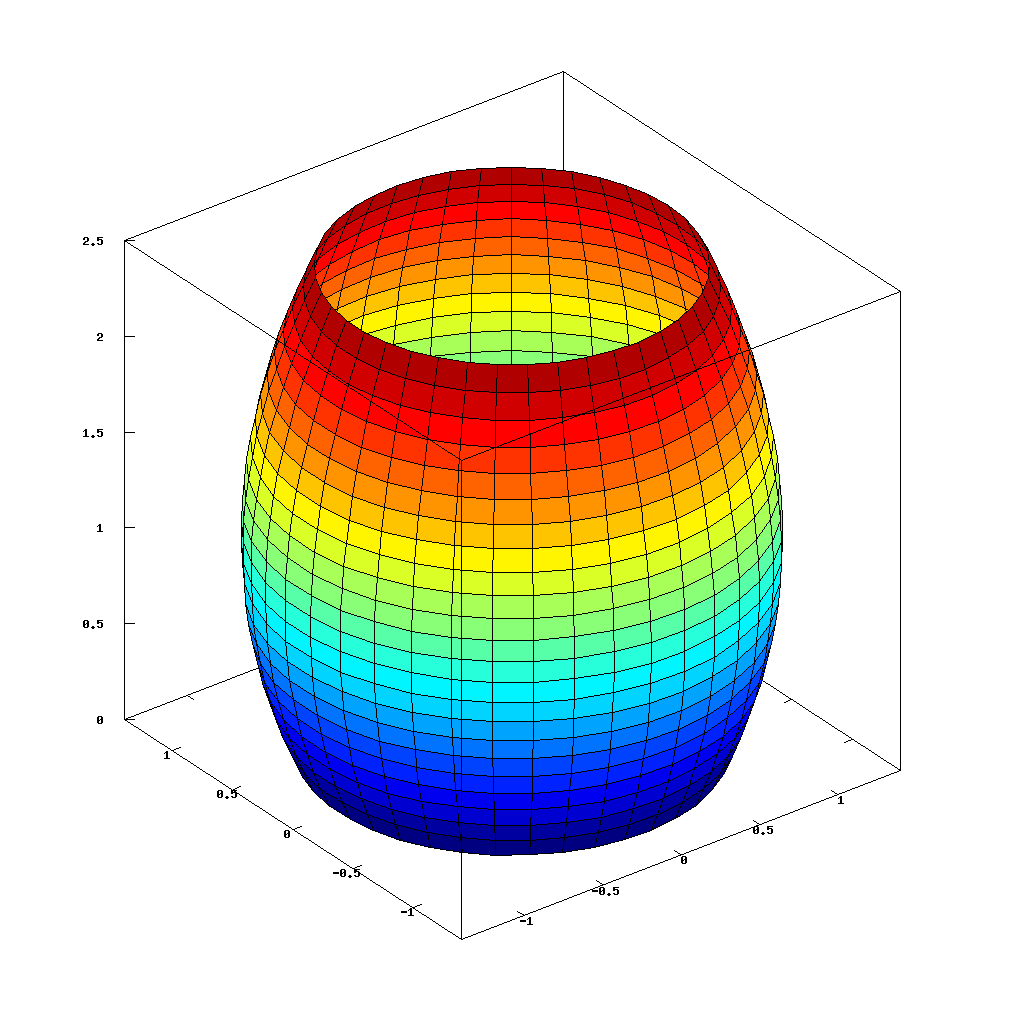
\includegraphics[height=300pt]{fig2}
\end{figure}

\newpage

\thispagestyle{empty}
\begin{abstract}
	\noindent I ett försök att rädda liv har vi undersökt hur vi kan säkra japanska hus vid jordbävningar genom att låta varje hus vila på flertalet pelare av speciell karaktär. Vi ämnar att med denna rapport analysera en speciell typ av sådan pelare, Beziér-pelaren. Vi kommer undersöka en sådan pelares stötdämpande förmåga med stort fokus på hur den beter sig under tryck. Vidare har vi funnit ekvationer som väldigt enkelt beskriver hur en sådan pelare förändras.
\end{abstract}

\newpage

\setcounter{page}{1}

\tableofcontents
\newpage

\section{Bakgrund}


	Vi har fått i uppgift skydda byggnader i områden ofta utsatta för jordbävningar. Dessa byggnader vilar på pelare med radien R=1 och höjden H=4 längdenheter. I båda ändar av pelaren, när den står under tryck, så finns det en glidförmåga som svarar till en glidkonstant G. Vi har blivit ålagda att undersöka det fall då  den undre glidkonstanten $G_1 = 0.4 $ och den övre glidkonstanten $G_2 = 0$.

\section{Problem}

För att kunna rita upp en pelare tänker vi oss att vi har en cylinder. Då denna ska kunna bukta gör vi en approximation av ytskitet med hjälp av en Beziér-kurva, för att råda bot på detta ickelinjära beteende. För att återskapa Beziér-kurvan behövs tre punkter. Start- och slutpunkt är redan givna så problemet är att bestämma styrpunkt. Ett givet krav på denna punkt är att vinkel mellan kurvan och marken hela tiden ska vara lika med vinkel mellan kurvan och pelarens tak. Pelaren har även olika radier i topp respektive botten. Detta gör det väldigt svårt att bestämma rätt styrpunkt. 

Den pelare vi har skapat kommer, då den blir utsatt för ett tryck, först att minska i area för att sedan vid någon speciell punkt börja expandera igen och därefter splittras sönder. Vi måste på något sätt kunna räkna oss fram till denna punkt.

\section {Egenskaper för radien i förhållande till glidkonstanten G}

	En formel för hur radien förändras beroende på bl. a. glidkonstanten G är given:
		$$r = R(1+G(\sqrt{\frac{H}{h}}-1)) $$

	$G=0$ medför $r = R$.

	Vi ämnar påvisa att perfekt glid ($G=1$) i båda ändar medför att pelaren inte bågnar utan blir en kort, knubbig cylinder. För att detta ska stämma så måste cylinderns volym med ny radie och ny höjd svara till den volym som finns från början.

	\begin{eqnarray*}
		\pi r^2 h &=& \pi R^2 H \\
		r^2 h &=& R^2 H \\
		(R(1+\sqrt{\frac{H}{h}}-1)^2*h &=& R^2 H \\
		(R \sqrt{\frac{H}{h}}) ^2*h &=& R^2 H \\
		R^2 \frac{H}{h}*h &=& R^2 H \\
		R^2 H &=& R^2 H \\
		VL &=& HL
	\end{eqnarray*}

	Eftersom denna likhet stämmer, och pelaren måste behålla konstant volym, så stämmer påståendet.

\section {Hitta styrpunkt för Bezier-kurva}
	\begin{figure}[htp]
	\centering
	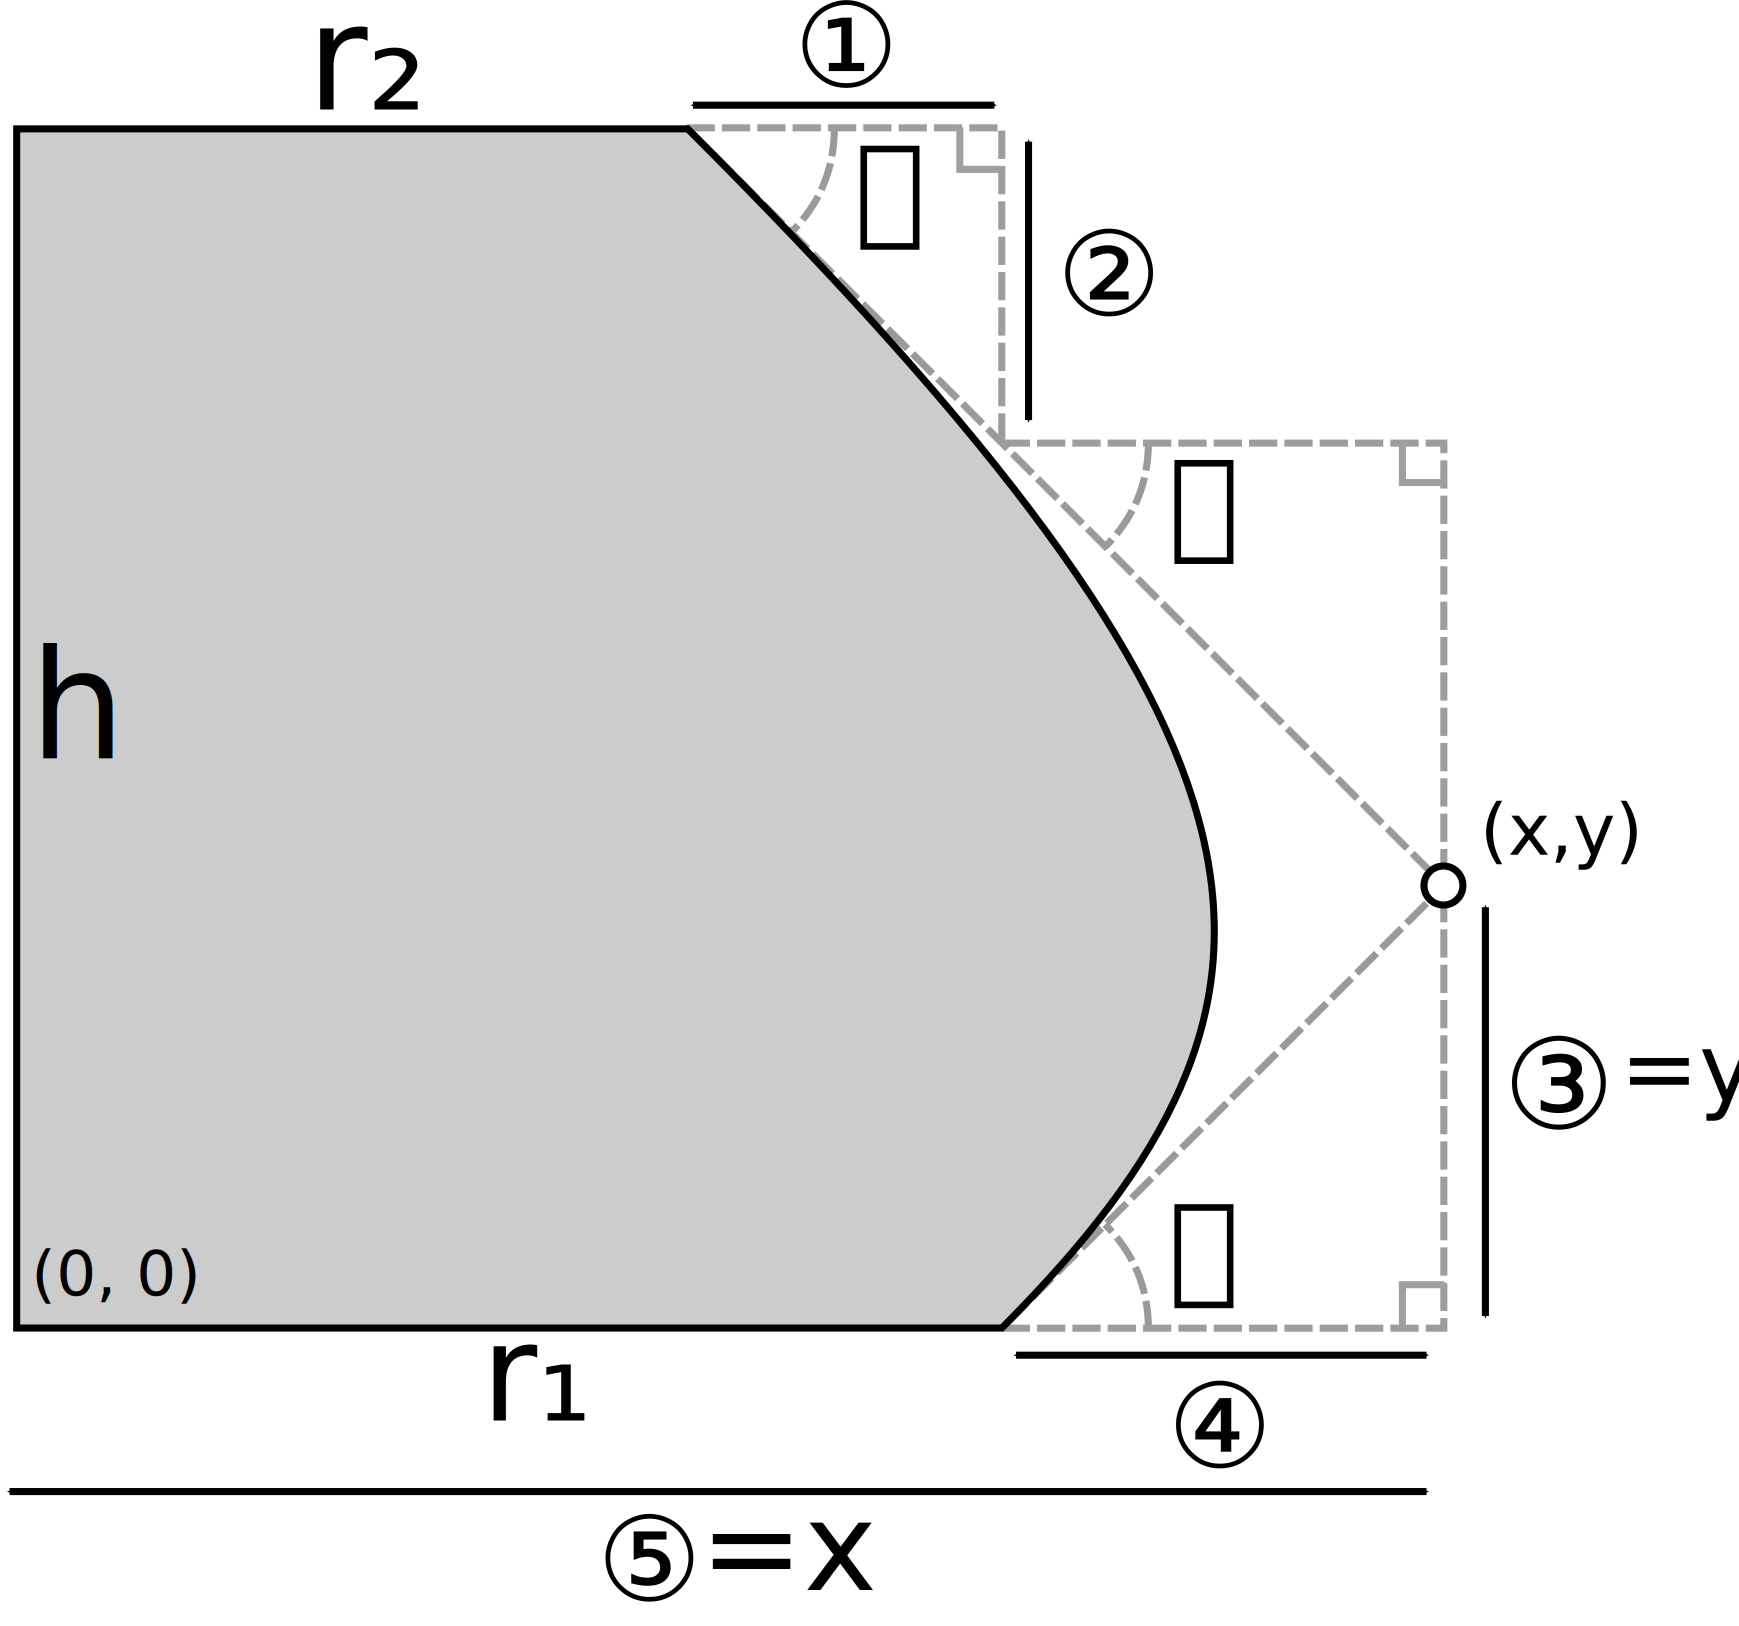
\includegraphics[width=280pt]{styrpunkt}
	\caption{Styrpunkt för bezierkurva}\label{fig:styrpunkt}
	\end{figure}

	Vi känner sedan tidigare till $h$, $r_1$ och $r_2$. Vinkeln till styrpunkten från bottenradien, $r_1$ är specifierad att vara samma som den från toppradien, $r_2$. Vi vet även att $r_2>r_1$. För att räkna ut var punkten kommer att sitta så måste vi först anta en vinkel, $\alpha$.

	Vi känner till både vinkeln och en av kateterna, $(1) = r_1-r_2$. Med hjälp av tangens kan vi då räkna ut den andra kateten, sträcka (2). Av symmetriskäl (vinkel $\alpha$ från båda håll) så vet vi att dubbla sträckan (3) är lika med $h-$ sträckan (2). Eftersom botten av pelaren ligger längs $x=0$ så har vi hittat att sträckan (3) är = Y-koordinaten för styrpunkten.

	Med hjälp av tangens igen får vi ut att vår sträcka (4), dvs styrpunktens avstånd från radien av bottenplattan, är sträckan (3) genom $tan(\alpha)$. För att hitta X-koordinaten för styrpunkten måste vi lägga på streckan för bottenradien $r_1$. Då får vi slutligen avståndet (4).

	\begin{eqnarray*}
		(1) &=& r_2-r_1 \\
		(2) &=& (1)*tan(\alpha) \\
	    y = (3) &=& \frac{h-(2)}{2} \\
		(4) &=& \frac{(3)}{tan(\alpha)} \\
	    x = (5) &=& r_1 + (4)
	\end{eqnarray*}

	\subsection{Volym och approximation av vinkeln}
	För att den här vinkeln ska stämma så måste volymen av den förtryckta pelaren vara samma som vid starttillfället då massan varken har gått förlorad eller ökat. Volymen för vår buktiga pelare får vi genom att integrera $ \int \pi x^2 z' dt $ över hela kurvans intervall, 0 till 1. 

	En vinkel svarar direkt mot en volym på pelaren. Lägre vinkel = mer buktande = större volym. Vid uträkning av styrpunkt och volym är radier och höjd kända, den enda variabel som påverkar denna volym är vinkeln. Den volym som vi får ut måste bli samma som originalpelarens volym, då materialet varken expanderas eller komprimeras.

	Volymen för originalpelaren fås av standardformeln för en cylinder, $ V=\pi r^2h + 2\pi r^2 $, där $h = H$ och $r = R$, dvs våra startvärden för höjd och radie av pelaren. Vi är intresserade av att hitta den vinkel där $V_{pelare} = V_{originalcylinder}$, dvs där $V_{pelare}-V_{originalcylinder} = 0$.

	Detta kan vi approximera med sekantmetoden. Genom att helt enkelt välja lämpliga startvinklar inom första kvadranten så itererar vi fram bättre approximationer av vinkeln tills dess att differensen är väldigt nära noll. Då har vi fått fram en bra approximation av vinkeln $\alpha$.

	\vspace{3mm}

	Det går att argumentera för att approximering med Newton-Raphson-metoden hade givit ett resultat snabbare, likväl som det går att argumentera för att expanderade möjligheter till kafferast är önskvärda.

\section{Motivation av använda formler}

\subsection{Volym}
$V=\int \pi x^2 z' dt$ är en formel som passar väldigt bra för för vår rotationskropp. Detta kan vi se genom analysera formeln lite. Vi ser att i våran figur är $z'=\frac{dz}{dt}$ dvs ett oändligt litet segment på z axeln med en viss höjd. Eftersom x beror på t, tiden, så kommer x variera och hela tiden utgöra radien av en cirkel runt z-axeln som sammanfaller med våran Beziér-kurva. Vi roterar nu denna punkt runt z axeln det ger oss en cirkel med radien x. \\

\begin{figure}[htp]
\centering
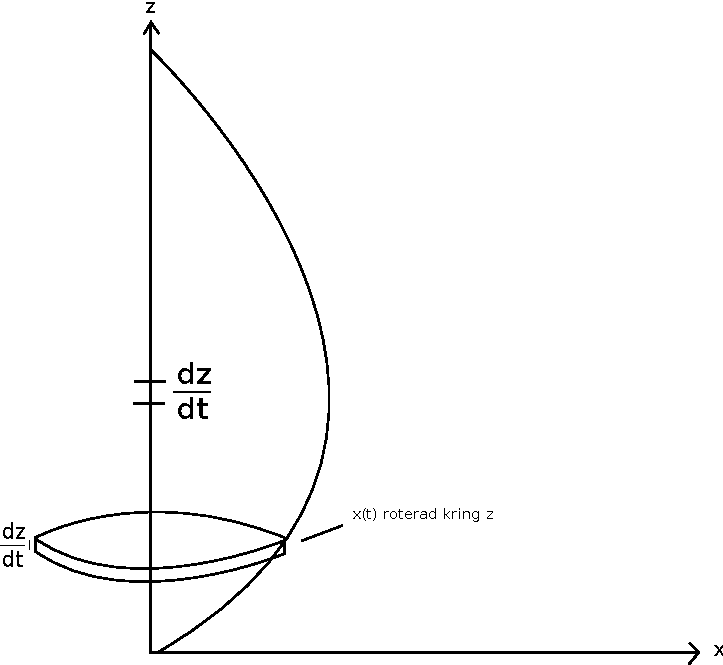
\includegraphics[scale=0.8]{volym}
\caption{rotationskropp}\label{fig:rotationskropp}
\end{figure}

Volymen av en cirkel ges av $V=\pi r^2 h$. Eftersom $ \frac{dz}{dt} $ är $\Delta$\emph{sträcka} längs z-axeln så kommer det motsvara höjden av cirkeln vi precis härledde. Det ger oss att volymen av en cirkel med oändligt liten höjd borde bli: $ V = \pi x^2 \frac{dz}{dt} $. Vi summerar nu ihop alla dessa cylindrar som befinner sig under våran kurva med en snygg integral:
$$V=\int \pi x^2 z' dt $$

\subsection{Area}
För att räkna ut arean av vår kropp behöver vi enbart modifiera vår ekvation litegrann. Istället för att summera volym element vill vi nu summera area element under vår kurva. Vi ser att vi kan approximera lutningen i varje punkt på kurvan genom: $ \sqrt{(x')^2+(x')^2} $ (figur nedan)

\begin{figure}[htp]
\centering
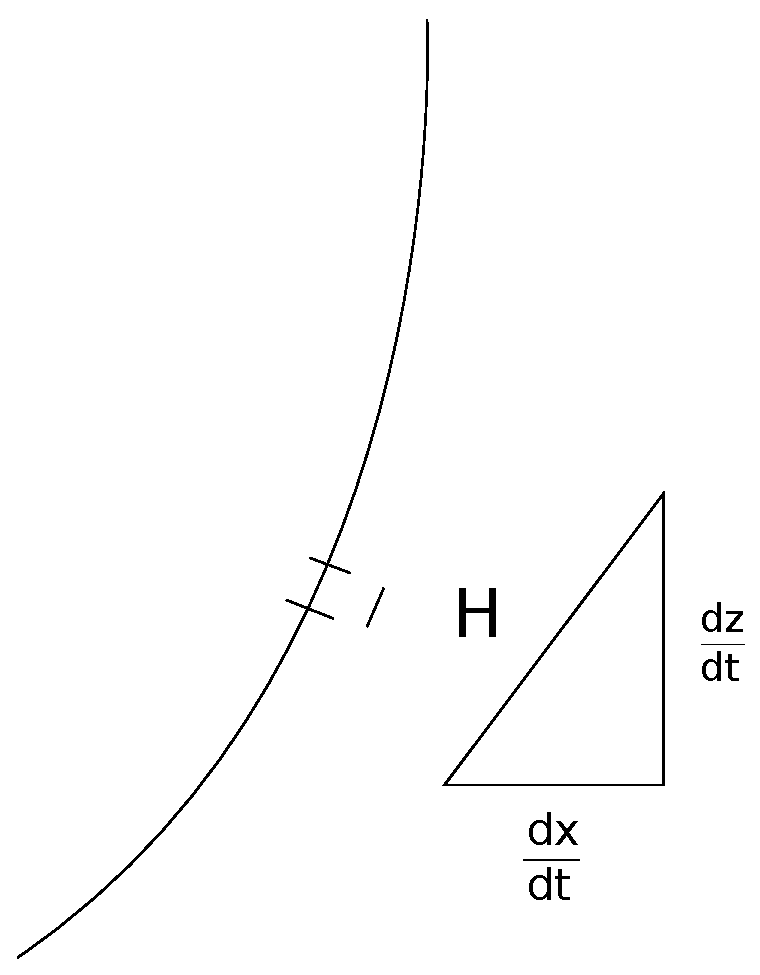
\includegraphics[scale=0.5]{area}
\caption{area element}\label{fig:area}
\end{figure}

Vilket stämmer väldigt bra överens med formeln för mantelytan hos en kon: $ A=2\pi s $ där $ s = \sqrt{(x')^2+(x')^2} $ vi summerar samtliga dessa element med avseende på t (förflyttningen längs vår Beziér-kurva) vilket ger oss en slutgiltig formel för area:
$$A=\int 2\pi x \sqrt{(x')^2 + (z')^2}  dt $$

\subsection{Polynomanpassning}
Vi är även intresserade av att enkelt kunna beskriva pelarens egenskaper och beteende vid olika tidpunkter. Enklast är att använda våra kunskaper inom analysen för att förstå hur vår kropp ändrar beteende med tiden. Ett polynom som beskriver vår kropp bra är följande:
$$F(h)=\frac{c_1}{h}+c_2 + c_3 h + c_4 h^2 $$

Detta då vi i polynomet ser de egenskaper vi vet att våran kropp har. Det första vi ser är att för små h värden växer sig första termen väldigt stor och är den dominerande termen i ekvationen. Dett syftar till att när pelare trycks ihop oändligt mycket så kommer ekvationen ge oss en oändlig area, helt i linje med förutsättningarna då pelaren sägs trasas sönder vid mindre h, vilket kan ses som en oändlig area (tänk: explosion utåt). Vi interpolerade med hjälp av minstakvadratmetoden de area värden vi fått från tidigare beräkningar.

$$ A\approx[31.4 , 29.9 , 28.6 , 27.5 , 27.3 , 29.7 , 39.1]$$

efter minstakvadratanpassning erhöll vi vårt polynom:
$$ P(x)= \frac{45.9}{h} - 20.4 + 14.7 h - 1.15 h^2 $$

\section{Numeriska metoder}
För uträkning av integraler använde vi oss uteslutande av quad funktionen. Då vi använde Octave\footnote{Fri implementation av matlab} har quad funktionen, till skillnad från matlabs originalinställning, väldigt bra tillförlitlighet. I de ekvationer vi använde fanns inga singulariteter så vi slapp även undan förbehandlig av integralerna.

\section{Slutsats}
Våran stackars pelare var behäftad med det felet att efter en viss kompression av arean åter börja expandera och strax efter den återfått ursprunglig area så kommer den tyvärr spricka sönder. Vi beräknar denna punkt med hjälp av vårat polynom genom användning av Newton-Raphsons metod:
$$ Brytpunkt:  h = 1.34934.. $$

Pelaren bör inte belastas mer än så att den trycks ihop till denna höjd, då den kommer att smula sönder. Vid en del belastning blir arean mindre och kan antas utsättas mindre för korrosion, eftersom den har en mindre yta som exponeras utåt, så möjligheten finns att lite tryck endast skulle göra pelaren väl.


\newpage
\section {Appendix}
	\subsection{Källkod}
	Källkoden finns bifogad separat pga. problem med paketet \emph{listings}.

	\subsection{Ihoptryckta pelare med styrpunkter}
	\begin{figure}[htp]
	\centering
	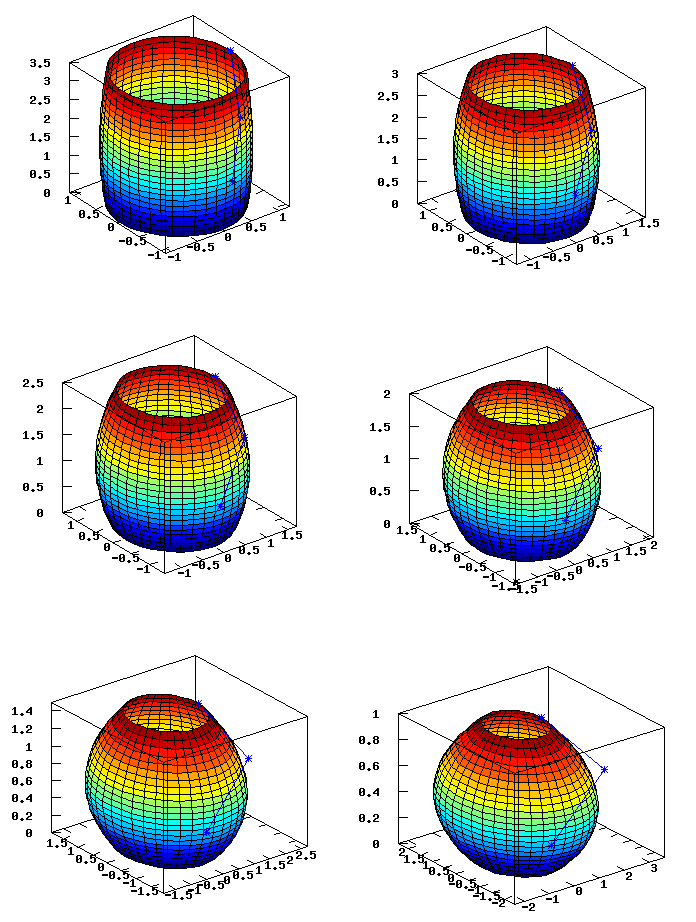
\includegraphics[width=320pt]{fig}
	%\caption{Ihoptryckt pelare och dess styrpunkt}\label{fig:fig}
	\end{figure}

	\newpage
	\subsection{Pelarens area i förhållande till dess höjd}
	\begin{figure}[htp]
	\centering
	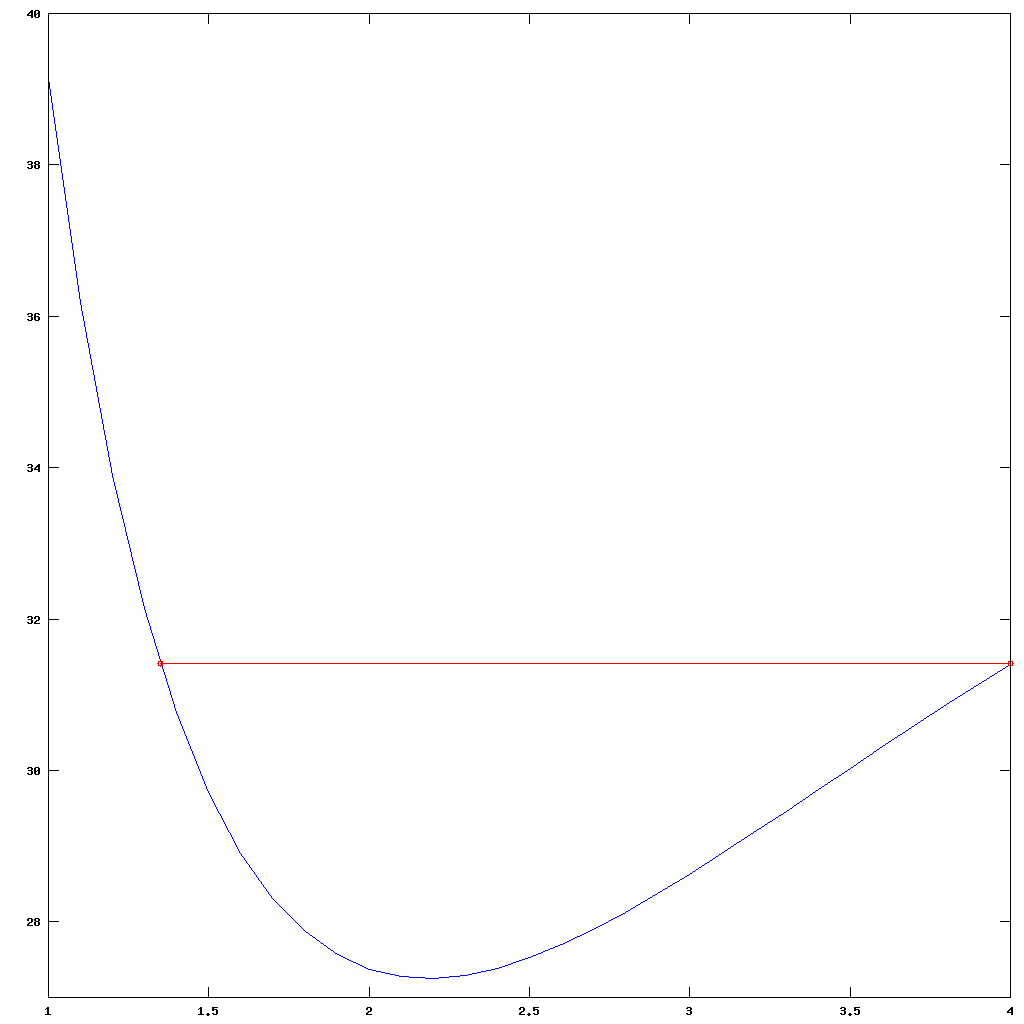
\includegraphics[width=320pt]{fig3}
	%\caption{Area i förhållande till höjd}\label{fig:fig3}
	\end{figure}

\end{document}
